

\documentclass{standalone}
\usepackage{tikz}
\usetikzlibrary{decorations.pathreplacing}
\usetikzlibrary{calc}
\usetikzlibrary{backgrounds} %特定的绘图操作置于背景层
\usetikzlibrary{3d}
\begin{document}
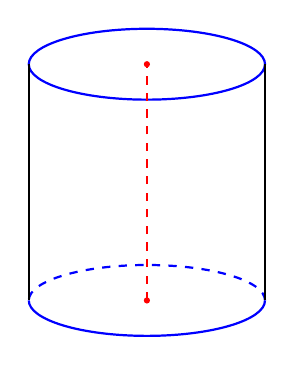
\begin{tikzpicture}[scale=1.5,
    y={(0cm,-0.3cm)}, % 设置 x 轴方向
    x={(1cm,0cm)},            % 设置 y 轴方向
    z={(0cm,1cm)}             % 设置 z 轴方向
]%斜二测画法
    % 定义圆柱的参数
    \def\radius{1} % 圆柱底面半径
    \def\height{2} % 圆柱的高度
        % 绘制顶面圆
        \begin{scope}
            %绘制一个圆
            % \draw(0,0,\height) circle (\radius);
            \draw [blue,thick] (\radius,0,\height) arc (0:-180:\radius) ;
            \draw [blue,thick] (\radius,0,\height) arc (0:180:\radius) ;
        \end{scope}

      
        % 绘制底面圆
        \begin{scope}
            \draw [blue,thick,dashed] (\radius,0,0) arc (0:-180:\radius) ;
            \draw [blue,thick] (\radius,0,0) arc (0:180:\radius) ;
        \end{scope}

        % 绘制母线
        \begin{scope}
            \draw[thick] (\radius,0,0) -- (\radius,0,\height);
            \draw[thick] (-\radius,0,0) -- (-\radius,0,\height);
        \end{scope}


        % 绘制高线
        \begin{scope}
        \fill[red] (0,0,0) circle (0.75pt);  % 绘制一个点测试一下 
        \fill[red] (0,0,\height) circle (0.75pt);  % 绘制一个点测试一下 
        \draw[thick,red,dashed] (0,0,0) -- (0,0,\height);


        \end{scope}

        % % 绘制括号
        % \begin{scope}[on background layer]
        %     \draw[decorate,decoration={brace,amplitude=10pt},thick] (0-0.1,0,0) -- (0-0.1,0,\height);
        % \end{scope}



\end{tikzpicture}
\end{document}